\documentclass[tikz]{standalone}
\begin{document}
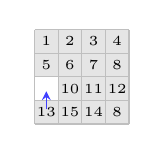
\begin{tikzpicture}[scale=.3]
\fill[gray!20] (0,0) rectangle (4,4);
\fill[white] (0,1) rectangle (1,2);
\draw[gray!50] (0,0) grid (4,4);
\node at (.5,3.5) {\tiny{1}};
\node at (1.5,3.5) {\tiny{2}};
\node at (2.5,3.5) {\tiny{3}};
\node at (3.5,3.5) {\tiny{4}};
\node at (.5,2.5) {\tiny{5}};
\node at (1.5,2.5) {\tiny{6}};
\node at (2.5,2.5) {\tiny{7}};
\node at (3.5,2.5) {\tiny{8}};
%\node at (.5,1.5) {\tiny{9}};
\node at (1.5,1.5) {\tiny{10}};
\node at (2.5,1.5) {\tiny{11}};
\node at (3.5,1.5) {\tiny{12}};
\node at (.5,.5) {\tiny{13}};
\node at (1.5,.5) {\tiny{15}};
\node at (2.5,.5) {\tiny{14}};
\node at (3.5,.5) {\tiny{8}};
\draw[shorten >=1pt,shorten <=1pt,blue!75,-stealth] (.5,.5) -- (.5,1.5);
\end{tikzpicture}
\end{document}